\documentclass[12pt,a4paper]{article}
\usepackage[utf8]{inputenc}
\usepackage[russian]{babel}
\usepackage{graphicx}
\usepackage{listings}
\begin{document}
\section{Рекомендуемая литература:}
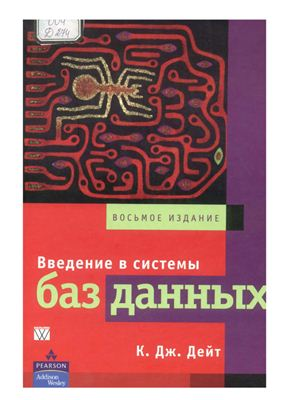
\includegraphics[width=4cm,height=5cm]{images/Overview/recommended_literature_book_01.jpg}
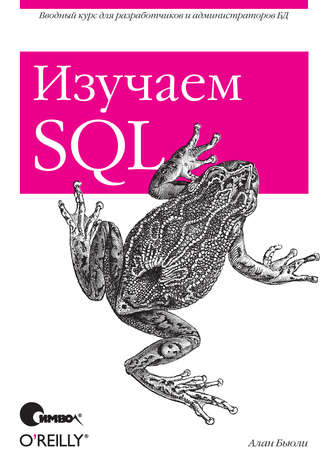
\includegraphics[width=4cm,height=5cm]{images/Overview/recommended_literature_book_02.jpg}
\begin{enumerate}
    \item Дейт К.Дж. Введение в системы баз данных
    \item Бьюли А. Изучаем SQL
    \item http://citforum.ru/database/
    \item https://dev.mysql.com/doc/
\end{enumerate}
\section{Необходимые инструменты:}
\begin{enumerate}
    \item MySQL Workbench https://dev.mysql.com/downloads/workbench/
    \item https://www.draw.io/
\end{enumerate}
\section{Темы лабораторных работ:}
\begin{enumerate}
    \item Проектирование базы данных. Описание предметной области, концептуальная, логическая модель базы данных. Нормализация.
    \item Физическая модель базы данных. Формулировка запросов к базе даных.
    \item Язык SQL. Создание таблиц. Оператор CREATE. Оптимизация используемых типов даных. Типы данных MySQL.
    \item Язык SQL. Выборка данных с использованием операторов Select. Where. Агрегаторы. Group By. Having. Order By.
    \item Язык SQL. Операторы Insert. Update. Delete. Условная логика IF, CASE.
    \item Язык SQL. Подзапросы. Несвязанные подзапросы. Связанные подзапросы. Размерность подзапроса.
    \item Язык SQL. Объединения.
    \item Оптимизация. Подсистемы хранения. Индексы. Explain. Типы индексов MySQL. 
    \item Базы данных дополнительные возможности. View. Тригеры. Хранимые процедуры.
    \item Защита данных. Транзакции. Уровни изоляции. Взаимные блокировки. Ручные блокировки.
    \item Администрирование баз данных. Системные таблицы. Переменные окружения. Права доступа пользователям. Логирование.
    \item Клиент-серверная архитектура. ORM. Hibernate. 
\end{enumerate}
\end{document}